\graphicspath{{system_design/fig/}}

\chapter{System Design}
\label{chap:system_design}

\begin{figure}[!h]
  \centering
  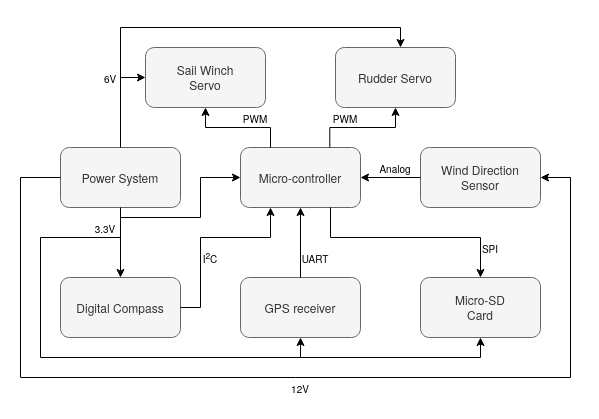
\includegraphics[width=0.918\linewidth]{system_diagram.png}
  \caption[System Diagram]{System Diagram}
  \label{fig:system_diagram}
\end{figure}

\section{Sail Vessel}
The sailing vessel houses the entire system illustrated in Fig. \ref{fig:system_diagram}. Designing and developing a sailboat is a complex task on its own, 
requiring expertise and experience in many fields, some of which include aerodynamics, hydrodynamics and material design. Given the complexity of this task 
and the time constraints of the project, an existing RC sailboat was used. A Dragonflite 95 RC sailboat\cite{Dragonflite} was modified to incorporate the system illustrated 
in Fig. \ref{fig:system_diagram}. The Dragonflite is 950 mm in length and has an overall weight of two kilograms. It features two sails (mainsail and jib),  
a carbon fibre mast and moulded carbon fibre keel with zinc alloy ballast bulb. The sailboat is operated
with a 2.4Ghz 4-channel digital proportional transmitter which communicates with a 2.4Ghz 4-channel receiver. The Dragonflite 95 comes preinstalled with a rudder 
servo motor as well as a sail winch servo motor. The sail winch servo controls both the mainsail 
and the jib simultaneously. The receiver and two servo motors are powered with a 6v battery source (4 AA batteries). The transmitter and receiver were 
removed as they are not needed in the development of a autonomous sailboat.

\section{Micro-controller}
Two options were considered for the micro-controller: the Adafruit BlackPill STM32F411 development board \cite{black_pill} and a Adafruit STM32F405 Feather \cite{STM32F405-specs}.
 The Adafruit BlackPill
has an Arm 32-bit Cortex-M4 CPU, which has a clock speed of 100MHz, 512KB flash memory, 128kB SRAM, and has a power efficiency
of $100\mu A$/$MHz$. The Adafruit feather has an Arm 32-bit Cortex-M4 CPU, with a clock speed of 168 MHz, 1MB flash memory, 
and has a power efficiency of $238\mu A$/$MHz$. Despite the higher price and power consumption of the Adafruit Feather, it was chosen for this system as it has a 
higher clock speed, which is needed for the navigational and control systems. The Adafruit feather also has a jst connection for a lithium-polymer battery as well as a 
3.3V regulator.


\section{Wind direction sensor}
The direction of apparent wind is needed to determine the optimal positioning of the sails. Wind direction sensors that were considered where: an ultrasonic 
anemometer, a mechanical wind vain, and the development of a wind direction sensor using four electret microphones and correlating the signals. The ultrasonic
anemometer that was considered was the WS303U by Sentec Meteorology, it was not used because it is too large for the sailing vessel. The development of a 
wind direction was not done because of the time constraints of the project. The mechanical wind vain was chosen as the most viable option. The sensor used was 
the FST200-202\cite{wind_sensor} made by firstrate sensor company. This sensor is designed for outdoor environments such as weather stations and boats, it therefore has 
excellent resistance to extreme weather conditions and erosion. The sensor works in wind speeds greater than 0.8 m/s, has a $22.5^{\circ}$ resolution and 
$\pm 3^{\circ}$ accuracy. It features automatic temperature compensation and operates in a temperature range of $-20^{\circ}C$ to $+85^{\circ}C$. The 
sensor has a working voltage of 12~30VDC, and its output is a 4-20 mA signal. 

\section{Servo motors}
Two servo motors are required: one for controlling the mainsail, and the other for controlling the rudder. The decision was made to use the preinstalled servo motors as 
the vessel was designed operate with these specific 
servo motors, it also keeps system design costs low. The manual specifies that a metal geared servo is used for rudder control
and a sail winch servo is used to control the sail position. Aside from this, no other information is given in the manual about the servo motors.  

\section{GPS receiver}
The GPS receiver is used to determine the GPS coordinates and speed of the sailing vessel. GPS coordinates of the vessel are needed to calculate the reference bearing 
(used in rudder control),
which is the bearing between current position and the target position. All GPS receivers on the market are accurate to within 2.5m, component choice is 
therefore dependant on factors such as price, power consumption and update rate.The GPS receiver that is used is a ATGM336H-5N\cite{GPS} module. It was chosen because it 
has a high tracking sensitivity, low power consumption and is low cost. Supply voltage of the receiver is 3.3V and it communicates via a UART interface. It has a 
tracking sensitivity of -162dBm, consumes $<25mA$ during continuous operation, 
has a first positioning time of 32 seconds, maximum update rate of 10Hz, and also features built in antenna short circuit protection.

\section{Digital compass}
The digital compass is used to determine the bearing of the sailing vessel, which is compared to the reference bearing to determine if the vessel is off course. It is 
required that the compass be able to perform tilt compensation, as the vessel will not always be on a level surface out at sea. The error in heading that occurs when tilt
compensation has not been implemented is illustrated in Fig.\ref{fig:tilt_error}, where it can be seen that as the pitch angle of the vessel increases, a greater error in 
heading occurs\cite{tilt_error}. To perform tilt compensation a magnetometer is needed to determine magnetic field vector, and a 
accelerometer is needed to determine the acceleration due to gravity vector. An IMU is a device that contains both a 3-axis magnetometer, 3-axis accelerometer and 3-axis gyroscope.
The two options that were considered were a AltIMU-10-V4\cite{altimu-10} made by Pololu Electronics and a MPU-9250/6500 9-axis IMU\cite{mpu-9250}. Both options feature 
16-bit ADC with signal conditioning. The 
Alt-IMU-10-V4 also features a digital barometer which is not needed for the purposes of this project. The MPU-9250/6500 was chosen for its low cost when compared 
to the AltIMU-10-V4. The MPU-9250/6500 has a supply voltage of 3.3V, an operating current of 3.5mA and an $I^{2}C$ interface.

\begin{figure}[!h]
  \centering
  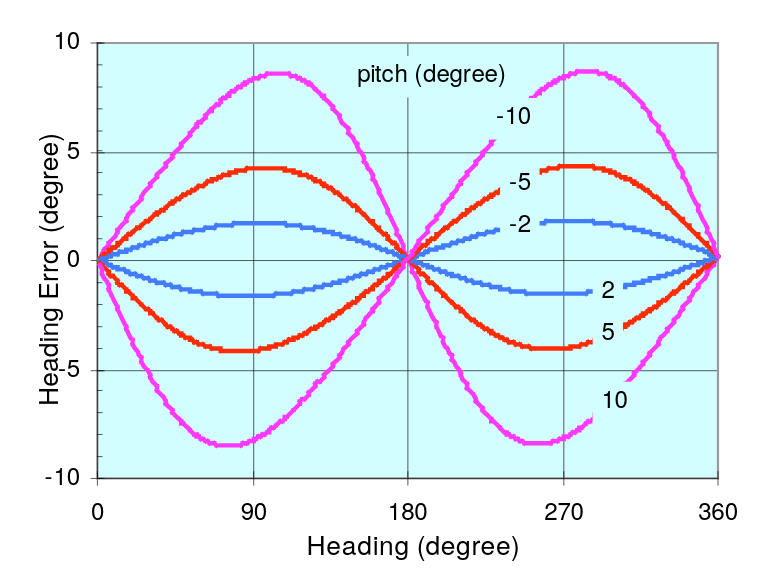
\includegraphics[width=0.5\linewidth]{tilt_error.png}
  \caption[Tilt error]{Heading error due to tilt without tilt compensation\cite{tilt_error}}
  \label{fig:tilt_error}
\end{figure}


\section{Micro-SD card}
The Micro-SD card is used for data-logging purposes, it allows for data from tests to be stored and analysed at a later time. Data that is logged during water tests 
include: current position, current bearing, desired bearing, bearing error, distance to target, wind direction, and tracking speed. A micro-Sd card socket made 
by Pololu\cite{sd} was used, and features a SPI.  


\section{Power system}
The power system consists of three separate power sources. The rudder servo and sail winch servo are powered by a 6v battery source consisting of four 1.5V
alkaline batteries in series. The Adafruit feather is powered by a 5000mAh 3.7V lithium polymer battery. The Adafruit feather is used to power the micro-SD 
card socket, GPS receiver, and digital compass. The wind direction sensor is powered with two 9V alkaline batteries in series. The use of one 12V power source 
with a 3.3V regulator was initially considered. Three separate power sources were chosen because the power consumption of the system is such that two 9V alkaline
batteries would only power the system for 2.13 hours, which was considered insufficient.
 %Discuss reason you used three
%different power sources instead of one. could say low cost?

\section{Metrics}


% \item Design and develop a digital compass that compensates for tilt.
% \item Determine and compare the accuracy of bearing obtained from a GPS receiver and that from a digital compass.
% \item System must be capable of logging operational data to a micro-SD card.
% \item Design and implement necessary navigational algorithms: Determine distance and bearing between two GPS coordinate.
% \item Design and develop sail control system.
% \item Design and develop rudder control system.
% \item Design and implement tacking manuever into system.

\subsubsection{Data logging}
To verify the system is capable of logging data as well as test the successful operation of the GPS receiver, a simple test is conducted. The experimental 
setup is as follows: The system is carried along a path, the GPS receiver will take samples at a rate of 1Hz, the GPS coordinates will then be logged to 
the micro-SD card on each sample, results are then analyzed to determine if path that was logged corresponds to the actual path travelled. 

\subsubsection{Digital compass}
Successful operation and accuracy of the digital compass is determined with two separate tests. 

The first test is done to test the accuracy of the digital 
compass. The setup is as follows: the digital compass undergoes extensive calibration; the digital compass as well as a handheld magnetic compass shown 
in Fig. \ref{}, are placed on a level piece of wood and 
spaced such that they do not interfere with each other; the wood is rotated in steps of $10^{\circ}$ anti-clockwise; each step readings from the handheld 
compass and the digital compass are taken and compared; because of the slight sample deviation present in the digital compass, an average of 10 samples
are taken for each step. 

The second test is done to determine the successful operation of the tilt compensation algorithm that is used. The 
setup is the same as the first test, but this time a pitch angle of $10^{\circ}$ is applied to the digital compass, the handheld compass is still placed 
flat. Again the wood is rotated in steps of $10^{\circ}$ anti-clockwise, and again ten samples are taken from the digital compass on each step, the average
of these samples is used for comparison. The results of this test are compared with the results from the first test - where the digital compass had a pitch 
and roll angle of zero. 

Accuracy of the digital compass needs to be compared with that of the GPS receiver. If the GPS receiver is capable of determining the bearing with better/or 
even the same degree of accuracy as that of the digital compass, then the use of a digital compass in the 
system does not make sense. It should be noted that the GPS receiver is only capable of determining bearing when the velocity of the system is greater than
zero. The test done to compare the accuracy of these two components is as follows: The GPS receiver is carried along a path of constant bearing and with a 
velocity similar to that of the maximum velocity the sailboat is capable of, bearing samples are then taken at a frequency of 1Hz, the same is then done 
for the digital compass, digital compass is held such that it points to the end point of the path throughout 
the test. The digital compass must be calibrated before the test. The results of the two tests are then compared.  

\subsubsection{Navigational calculations}
The successful operation of the algorithm used to determine distance between two points is verified using the following experimental setup: a target GPS 
coordinate is given to the system, the current GPS coordinates are obtained from the GPS receiver at varying distances from the target and distance is 
calculated, distances that samples are taken are physically measured out before the test is done, an average of ten distance calculations are done for each
change in distance. 

% Should include test to verify bearing here?

\subsubsection{Sail control}
A test will be conducted to verify accuracy as well as successful operation of the sail control system. The experimental setup is as follows: wind direction 
sensor will be adjusted in $22.5^{\circ}$ increments - wind sensor's resolution - with $0^{\circ}$ corresponding to center on no sail-zone, corresponding 
change in sail position will then be measured from the centerline of the boat.

\subsubsection{Rudder control}
The first test will test the operation of the rudder control out of the water. A target GPS coordinate will be chosen and given to the system, the system 
will then be carried along a path of constant bearing ending in the target coordinate, the current position, desired bearing, actual bearing and error signal
will be logged throughout the test. 

The second test will be done on the dam by the Maties canoe club. The experimental setup is as follows: a target coordinate is programmed into the system,
the digital compass is calibrated and the sailboat is placed at a suitable starting location. Apparent wind is determined beforehand and the sail position is 
set accordingly (sail position control will be disabled for this test). The data that will be logged throughout the test is: current GPS coordinate, distance 
to target, desired heading, actual heading, heading error signal, rudder PWM value and apparent wind direction. The purpose of this test is to evaluate the performance
of the rudder controller and determine optimal gains through experimentation, this test will therefore be repeated more than once.

\subsubsection{Sytem}
A similar test will be done on water at the Maties canoe club to verify the successful operation of the entire system - navigational and control systems. The test
is similar to the second test done for the rudder control except the sail control will be included, and the setup is as follows: a target coordinate is 
programmed into the system and the digital compass is calibrated, the sailboat is placed at a suitable starting point, data will be logged throughout the test. 
The data that is logged is: current GPS coordinate, distance to target, desired bearing, actual bearing, bearing error signal, rudder servo PWM value, apparent 
wind direction, sail position value, sail servo PWM value.

The final test will have the same experimental setup as the previous test, only difference being that two separate waypoints will be set beforehand. This test is 
done to verify the vessels ability to navigate to a single waypoint and then change navigation to a different waypoint. 






